\documentclass[aspectratio=169]{beamer}

\usetheme{default}
\setbeamertemplate{navigation symbols}{}
\setbeamertemplate{enumerate item}{\color{navy}\arabic{enumi}.}
\setbeamertemplate{itemize item}{\color{black}\textbullet}
\setbeamertemplate{itemize subitem}{\color{black}\textbullet}
\usepackage{booktabs}
\usepackage{xcolor}
\usepackage{tikz}
\usetikzlibrary{shapes,arrows,positioning}
\definecolor{navy}{RGB}{0, 0, 128}
\definecolor{lightblue}{RGB}{230,240,250}
\definecolor{darkgreen}{RGB}{0,100,0}
\definecolor{lightgreen}{RGB}{230,250,230}
\newcommand{\highlight}[1]{\colorbox{lightblue}{$\displaystyle\textcolor{navy}{#1}$}}
\newcommand{\highlighttext}[1]{\colorbox{lightblue}{\textcolor{navy}{#1}}}
\newcommand{\highlightgreen}[1]{\colorbox{lightgreen}{$\displaystyle\textcolor{darkgreen}{#1}$}}



\begin{document}

\begin{frame}

CCPs don't simplify counterfactual simulations

\bigskip{}

\onslide<2->{
Why? We don't observe $\ln p_{kt+1}$ in the counterfactual world
}

\bigskip{}

\onslide<3->{
If we could observe it, we wouldn't need a structural model to begin with
}


\end{frame}





\begin{frame}

\onslide<1->{
Worst case: must solve full backwards recursion or fixed point problem once
}

\bigskip{}

\onslide<2->{
When policy expires after $t$ periods, CCPs remain valid at $t+1$
}

\bigskip{}

\onslide<3->{
This means: only need to solve model for periods when policy is in place
}

\bigskip{}

\onslide<4->{
Examples: tuition subsidies, home-owner subsidies, G.W. Bush tax cuts (2001, 2003)
}

\end{frame}


\begin{frame}
\centering
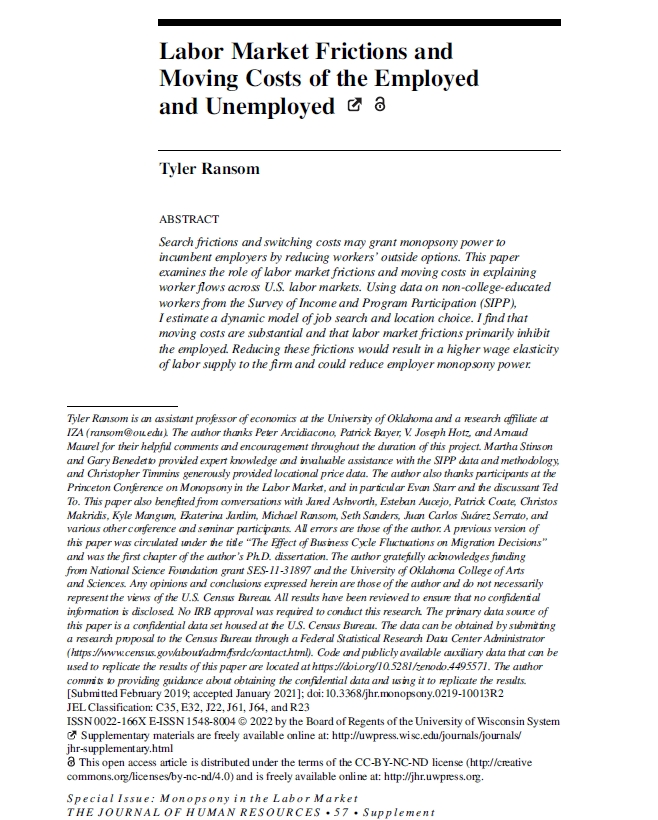
\includegraphics[width=0.5\textwidth]{Ransom2022_cover.jpg}
\end{frame}



\begin{frame}

\onslide<1->{
Ransom (2022) estimates a dynamic migration model using CCP methods
}

\bigskip{}

\onslide<2->{
\textcolor{navy}{Counterfactual simulations:}
\bigskip\par
\begin{itemize}
\itemsep1.5em
\item Earnings shocks (local vs spatially correlated)
\item Unemployment shocks (local vs spatially correlated)
\item Moving subsidy (\$10,000)
\end{itemize}
}

\bigskip{}

\onslide<3->{
\textcolor{navy}{Key restriction:} Only temporary policies (one year)
}

\bigskip{}

\onslide<4->{
Why? Future value terms ($\ln p_{kt+1}$) from CCP estimation not valid beyond $t+1$
}

\bigskip{}

\onslide<5->{
Longer counterfactuals require full value function solution (computationally infeasible)
}

\end{frame}



\end{document}